\renewcommand*\chappic{img/hashalgos.pdf}
\renewcommand*\chapquote{}
\renewcommand*\chapquotesrc{}
%
\chapter{Hash algorithms}
\label{ch:hash}

In this chapter we will define hash functions and their desired security
properties. Followingly we look at SHA256 and MD4 as established hash functions.
We will represent them with Boolean algebra (in chapter~\ref{ch:enc}) to make
it possible to reason about states in those hash functions using SAT solvers.

\section{Preliminaries Redux}
\label{sec:hash-prelim}
%
\index{Hash value}
\index{Preimage}
\index{Hash function}
\begin{defi}[Hash function]
  A \emph{hash function} is a mapping $h: X \to Y$ with $X = \left\{0,1\right\}^*$ and
  $Y = \left\{0,1\right\}^n$ for some fixed $n \in {\symbol{"2115}}_{\geq 1}$.  % FAIL
  \begin{itemize}[noitemsep,topsep=0pt]
    \item Let $x \in X$, then $h(x)$ is called \emph{hash value of $x$}.
    \item Let $h(x) = y \in Y$, then $x$ is called \emph{preimage of $y$}.
  \end{itemize}
\end{defi}

Hash functions are considered as cryptographic primitives
used as building blocks in cryptographic protocols.
A hash function has to satisfy the following security requirements:

\index{Preimage resistance}
\begin{defi}[Preimage resistance]
  Given $y \in Y$,
  a hash function $h$ is \emph{preimage resistant} iff it is computationally infeasible
  to find $x \in X$ such that $h(x) = y$.
\end{defi}

\clearpage
\index{Second-preimage resistance}
\begin{defi}[Second-preimage resistance]
  Given $x \in X$,
  a hash function $h$ is \emph{second-preimage resistant} iff it is computationally infeasible
  to find $x_2 \in X$ with $x \neq x_2$ such that $h(x) = h(x_2)$.
  $x_2$ is called \emph{second preimage}.
\end{defi}

\index{Collision resistance}
\index{Collision}
\begin{defi}[Collision resistance]
  A hash function $h$ is \emph{collision resistant} iff it is computationally infeasible to
  find any two $x \in X$ and $x_2 \in X$ with $x \neq x_2$ such that $h(x) = h(x_2)$.
  Tuple $(x, x_2)$ is called \emph{collision}.
\end{defi}

As far as hash functions accept input strings of arbitrary length, but return a fixed
size output string, existence of collisions is unavoidable~\cite{schlaffer}.
However, good hash functions make it very difficult to find collisions or preimages.

Any digital data can be hashed (i.e. used as input to a hash function) by considering
it in binary representation. The format or encoding is not part of the hash function's
specification.

\subsection{Merkle-Damg\aa{}rd designs}
\label{sec:hash-md}
%
The Merkle-Damg\aa{}rd design is a particular design of hash functions providing the
following security guarantee:

\begin{defi}[Collision resistance inheritance]
  Let $F_0$ be a collision resistant compression function.
  A hash function in Merkle-Damg\aa{}rd design is collision resistant if $F_0$ is collision resistant.
\end{defi}

This motivates thorough research of collisions in compression functions.
The design was found independently by Ralph C. Merkle and Ivan B. Damg\aa{}rd.
It was described by Merkle in his PhD thesis~\cite[p. 13--15]{merkle1979secrecy}
and followingly used in popular hash functions such as MD4, MD5 and the SHA2 hash function family.
The single-pipe design works as follows:
\begin{enumerate}\itemsep0pt
\item Split the input into blocks of uniform block size.
  If necessary, apply padding to the last block to achieve full block size.
\item Compression function $F_0$ is applied iteratively using the output $y_{i-1}$ of
  the previous iteration and the next input block $x_i$, denoted $y_i = F_0(y_{i-1}, x_i)$.
\item An optional postprocessing function is applied.
\end{enumerate}

\subsection{Padding and length extension attacks}
\label{sec:hash-length-ext-attack}
%
Hash functions of single-piped Merkle-Damg\aa{}rd design inherently suffer
from length extension attacks. MD4 and SHA256 apply padding to their input
to normalize their input size to a multiple of its block size.
The compression function is applied afterwards. This design is vulnerable
to length extensions.

Consider some collision $(x_0, x_1)$ with $F_0(x_0) = y = F_0(x_1)$ where $x_0$ and
$x_1$ have a size of one block. Let $p$ be a suffix with size of one block.
Then also $(x_0 \,\|\, p, x_1 \,\|\, p)$ (where $\|$ denotes concatenation)
represents a collision in single-piped Merkle-Damg\aa{}rd designs, because
it holds that:
\[ F_0(F_0(x_0), p) = F_0(F_0(x_1), p) \iff F_0(y, p) = F_0(y, p) \]
Hence $(x_0 \,\|\, p, x_1 \,\|\, p)$ is a collision as well.
As far as $F_0$ is applied recursively to every block, $p$ can be of arbitrary size
and $(x_0, x_1)$ can be of arbitrary uniform size.

Because of this vulnerability, cryptanalysts only need to find a collision
in compression functions. In our tests will only consider input of one block
and padding will be neglected due to this vulnerability.

\subsection{Example usage}
\label{sec:hash-usage}
%
One example showing the use of hash functions as primitives are JSON Web Tokens (JWT)
specified in RFC~7519~\cite{rfc7519}. Its application allows web developers to
represent claims to be transferred between two parties.

Section~8 defines implementation requirements and refers to RFC~7518~\cite{rfc7518},
which specifies cryptographic algorithms such as \enquote{HMAC SHA-256} to be
implemented. It is (besides \enquote{none}) the only required signature and MAC algorithm.

\section{MD4}
\label{sec:dc-md4}
%
\index{MD4}
MD4 is a cryptographic hash function originally described in RFC~1186~\cite{rfc1186},
updated in RFC~1320~\cite{rfc1320} and declared obsolete by RFC~6150~\cite{rfc6150}. It was
invented by Ronald Rivest in 1990 with properties given in Table~\ref{tab:md4}.
In 1995~\cite{Dobbertin1998} successful full-round attacks have been found to break collision resistance.
Followingly preimage and second-preimage resistance in MD4 have been broken as well.
Some of those attacks are described in~\cite{md4-2007} and \cite{cryptoeprint:2005:151}.
We derived a Python~3 implementation based on a Python~2 implementation
and made it available on github~\cite{md4-py3k}.

\begin{table}[h]
  \begin{center}
    \begin{tabular}{lcl}
      block size           & 512 bits       & namely variable \texttt{block} in RFC~1320~\cite{rfc1320} \\
      digest size          & 128 bits       & as per Section~3.5 in RFC~1320~\cite{rfc1320} \\
      internal state size  & 128 bits       & namely variables $A$, $B$, $C$ and $D$ \\
      word size            & 32 bits        & as per Section~2 in RFC~1320~\cite{rfc1320} \\
    \end{tabular}
    \caption{MD4 hash algorithm properties}
    \label{tab:md4}
  \end{center}
\end{table}

MD4 uses three auxiliary Boolean functions:
\begin{defi}
  The Boolean \boolf{IF} function is defined as follows:
  If the first argument is true, the second argument is returned.
  Otherwise the third argument is returned.

  The Boolean \boolf{MAJ} function returns true if the number
  of Boolean values true in arguments is at least $2$.
  The Boolean \boolf{XOR} function returns true if the number
  of Boolean values true in arguments is odd.
\end{defi}

Using the logical operators $\land$ (AND), $\lor$ (OR) and $\neg$ (NEG)
we can define them as (see section~\ref{sec:sat-intro} for a thorough
discussion of these operators):
\begin{align}
  \IF(X,Y,Z) &\coloneqq (X \land Y) \lor (\neg X \land Z) \\
  \MAJ(X,Y,Z) &\coloneqq (X \land Y) \lor (X \land Z) \lor (Y \land Z) \\
  \XOR(X,Y,Z) &\coloneqq (X \land \neg Y \land \neg Z) \lor (\neg X \land Y \land \neg Z) \nonumber\\
              &\lor (\neg X \land \neg Y \land Z) \lor (X \land Y \land Z) \nonumber\\
              &\coloneqq (X \oplus Y \oplus Z)
\end{align}


In the following a brief overview over MD4's design is given.

\begin{description}
  \item[Padding and length extension.]
    First of all, padding is applied. A single bit $1$ is appended to the
    input. As long as the input does not reach a length congruent 448 modulo 512,
    bit $0$ is appended.
    Followingly, length appending takes place. Represent the length of the input
    (without the previous modifications) in binary and take its first
    64 less significant bits. Append those 64 bits to the input.
  \item[Initialization.]
    The message is split into 512-bit blocks (i.e. 16 32-bit words).
    Four state variables $A_{i}$ with $-4 \leq i < 0$ are initialized with these
    hexadecimal values:
    % remark: A_{-4} := A, A_{-1} := B, A_{-2} := C, A_{-3} := D on Wikipedia
    \[
      \mathtt{[A_{-4}]}\; \texttt{01234567} \quad
      \mathtt{[A_{-1}]}\; \texttt{89abcdef} \quad
      \mathtt{[A_{-2}]}\; \texttt{fedcba98} \quad
      \mathtt{[A_{-3}]}\; \texttt{76543210}
    \]
  \item[Round function with state variable updates.]
    The round function is applied in three rounds with 16 iterations.
    In every iteration values $A_{-1}$, $A_{-2}$ and $A_{-3}$ are taken
    as arguments to function $F$. Function $F$ is \boolf{IF} in round~1,
    followed by \boolf{MAJ} for round~2 and \boolf{XOR} for the final round~3.
    The resulting value is added to $A_{-1}$, current message block $M$
    and constant $X$. Finally the 32-bit sum will be left-rotated by $p$
    positions. Left rotation is formally defined in Definition~\ref{def:shifts}.
    The values of $X$ and $p$ are defined as follows:

    Let $i$ be the iteration counter between $1$ and $16$ and
    $r$ the round between $1$ and $3$. Then $X$ takes the value
    of the $i$-th column and $r$-th row of matrix $C$.
    $p$ takes the value of row $r$ and column $i \bmod{4}$ of matrix $P$.
    
    \[
      C = \left(\begin{array}{cccccccccccccccc}
        0 & 1 & 2 & 3 & 4 & 5 & 6 & 7 & 8 & 9 & 10 & 11 & 12 & 13 & 14 & 15 \\
        0 & 4 & 8 & 12 & 1 & 5 & 9 & 13 & 2 & 6 & 10 & 14 & 3 & 7 & 11 & 15 \\
        0 & 8 & 4 & 12 & 2 & 10 & 6 & 14 & 1 & 9 & 5 & 13 & 3 & 11 & 7 & 15
      \end{array}\right)
    \] \[
      P = \begin{pmatrix}
        3 & 7 & 9 & 11 \\
        3 & 5 & 9 & 13 \\
        3 & 9 & 11 & 15
      \end{pmatrix}
    \]

    This round function design is visualized in Figure~\ref{fig:md4-round-function}.
\end{description}

\begin{figure}[p]
  \begin{center}
    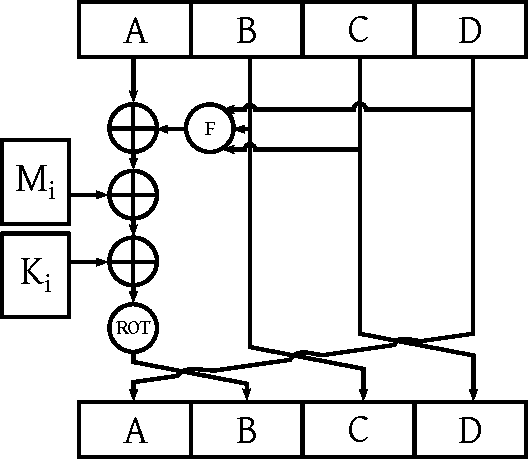
\includegraphics{img/md4.pdf}
    \caption{MD4 round function updating state variables}
    \label{fig:md4-round-function}
  \end{center}
%\end{figure}
%\begin{figure}[p]
  \begin{center}
    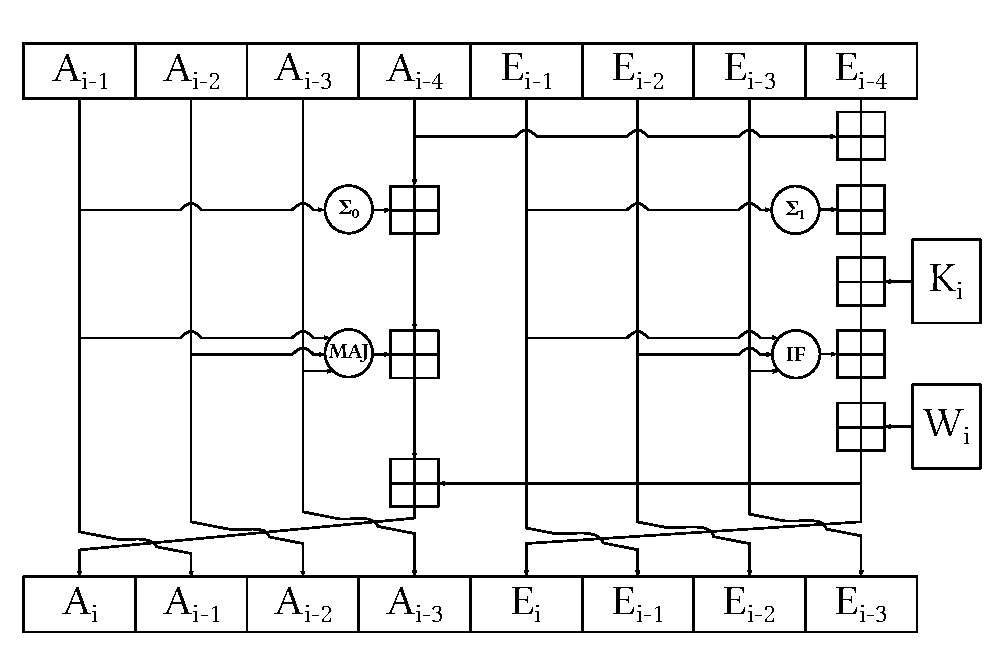
\includegraphics[width=\textwidth]{img/sha256.pdf}
    \caption{SHA-256 round function as characterized in~\cite{analysisSHA256}}
    \label{fig:sha256-round-function}
  \end{center}
\end{figure}










\section{SHA-256}
\label{sec:dc-sha-256}
%
\index{SHA-256}
SHA-256 is a hash function from the SHA-2 family designed by the National Security Agency (NSA)
and published in 2001~\cite{fips-pub-180-4}. It uses a Merkle-Damg\aa{}rd construction
with a Davies-Meyer compression function. The best known preimage attack was found in 2011
and breaks preimage resistance for 52~rounds~\cite{bicliques}. The best known collision attack
breaks collision resistance for 31~rounds of SHA-256~\cite{improving} and pseudo-collision
resistance for 46~rounds~\cite{high2011}.

\begin{table}[!hb]
  \begin{center}
    \begin{tabular}{lcl}
      block size           & 512 bits   & as per Section~1 of the standard~\cite{fips-pub-180-4} \\
      digest size          & 256 bits   & mentioned as Message Digest size~\cite{fips-pub-180-4} \\
      internal state size  & 256 bits   & as per Section~1 of the standard~\cite{fips-pub-180-4} \\
      word size            & 32 bits    & as per Section~1 of the standard~\cite{fips-pub-180-4}
    \end{tabular}
    \caption{SHA-256 hash algorithm properties}
    \label{tab:sha256}
  \end{center}
\end{table}
%
\index{Left-shift}
\index{Right-shift}
\index{Left-rotation}
\index{Right-rotation}
\begin{defi}[Shifts, rotations and a notational remark]
  \label{def:shifts}
  Consider a 32-bit word $X$ with 32 binary values $b_i$ with $0 \leq i \leq 31$.
  $b_0$ refers to the least significant bit. Shifting ($≪$ and $≫$) and
  rotation ($⋘$ and $⋙$) creates a new 32-bit word $Y$ with 32 binary values $a_i$.
  We define the following notations:
  \begin{align*}
    Y \coloneqq X ≪ n  &\iff a_i \coloneqq b_{i-n} \text{ if } 0 \leq i-n < 32 \text{ and } 0 \text{ otherwise } \\
    Y \coloneqq X ≫ n  &\iff a_i \coloneqq b_{i+n} \text{ if } 0 \leq i+n < 32 \text{ and } 0 \text{ otherwise } \\
    Y \coloneqq X ⋘ n  &\iff a_i \coloneqq b_{i-n \bmod{32}} \text{ as used in MD4} \\
    Y \coloneqq X ⋙ n  &\iff a_i \coloneqq b_{i+n \bmod{32}}
  \end{align*}
\end{defi}
%
Besides MD4's \boolf{MAJ} and \boolf{IF},
another four auxiliary functions are defined. Recognize that $\oplus$ denotes
the XOR function whereas $\boxplus$ denotes 32-bit addition.
\[
  \begin{array}{rcccccl}
    \Sigma_0(X) &\coloneqq& (X ⋙ 2) &\oplus& (X ⋙ 13) &\oplus& (X ⋙ 22) \\
    \Sigma_1(X) &\coloneqq& (X ⋙ 6) &\oplus& (X ⋙ 11) &\oplus& (X ⋙ 25) \\
    \sigma_0(X) &\coloneqq& (X ⋙ 7) &\oplus& (X ⋙ 18) &\oplus& (X ≫ 3) \\
    \sigma_1(X) &\coloneqq& (X ⋙ 17) &\oplus& (X ⋙ 19) &\oplus& (X ≫ 10)
  \end{array}
\]
%
\begin{description}
  \item[Padding and length extension.]
    The padding and length extension scheme of MD4 is used also in SHA-256.
    Append bit $1$ and followed by a sequence of bit $0$ until the message reaches a length
    of 448 modulo 512 bits. Afterwards the first 64 bits of the binary representation
    of the original input are appended.
  \item[Initialization.]
    In a similar manner to MD4, initialization of internal state variables
    (called \enquote{working variables} in~\cite[Section~6.2.2]{fips-pub-180-4})
    takes place before running the round function. The eight state variables
    are initialized with the following hexadecimal values:
    \[
      \begin{array}{llll}
        A_{-1} = \texttt{6a09e667} &
        A_{-2} = \texttt{bb67ae85} &
        A_{-3} = \texttt{3c6ef372} &
        A_{-4} = \texttt{a54ff53a} \\
        E_{-1} = \texttt{510e527f} &
        E_{-2} = \texttt{9b05688c} &
        E_{-3} = \texttt{1f83d9ab} &
        E_{-4} = \texttt{5be0cd19}
      \end{array}
    \]
    Furthermore SHA-256 uses 64 constant values in its round function.
    We initialize step constants $K_i$ for $0 \leq i < 64$ with the following hexadecimal
    values (which must be read left to right and top to bottom):
    \[
      \begin{array}{cccccc}
        \texttt{428a2f98} & \texttt{71374491} & \texttt{b5c0fbcf} & \texttt{e9b5dba5} & \texttt{3956c25b} & \texttt{59f111f1} \\
        \texttt{923f82a4} & \texttt{ab1c5ed5} & \texttt{d807aa98} & \texttt{12835b01} & \texttt{243185be} & \texttt{550c7dc3} \\
        \texttt{72be5d74} & \texttt{80deb1fe} & \texttt{9bdc06a7} & \texttt{c19bf174} & \texttt{e49b69c1} & \texttt{efbe4786} \\
        \texttt{0fc19dc6} & \texttt{240ca1cc} & \texttt{2de92c6f} & \texttt{4a7484aa} & \texttt{5cb0a9dc} & \texttt{76f988da} \\
        \texttt{983e5152} & \texttt{a831c66d} & \texttt{b00327c8} & \texttt{bf597fc7} & \texttt{c6e00bf3} & \texttt{d5a79147} \\
        \texttt{06ca6351} & \texttt{14292967} & \texttt{27b70a85} & \texttt{2e1b2138} & \texttt{4d2c6dfc} & \texttt{53380d13} \\
        \texttt{650a7354} & \texttt{766a0abb} & \texttt{81c2c92e} & \texttt{92722c85} & \texttt{a2bfe8a1} & \texttt{a81a664b} \\
        \texttt{c24b8b70} & \texttt{c76c51a3} & \texttt{d192e819} & \texttt{d6990624} & \texttt{f40e3585} & \texttt{106aa070} \\
        \texttt{19a4c116} & \texttt{1e376c08} & \texttt{2748774c} & \texttt{34b0bcb5} & \texttt{391c0cb3} & \texttt{4ed8aa4a} \\
        \texttt{5b9cca4f} & \texttt{682e6ff3} & \texttt{748f82ee} & \texttt{78a5636f} & \texttt{84c87814} & \texttt{8cc70208} \\
        \texttt{90befffa} & \texttt{a4506ceb} & \texttt{bef9a3f7} & \texttt{c67178f2}
      \end{array}
    \]
  \item[Precomputation of W.]
    Let $W_i$ for $0 \leq i < 16$ be the sixteen 32-bit words of the padded input message.
    Then compute $W_i$ for $16 \leq i < 64$ the following way:
    \[ W_i \coloneqq \sigT(W_{i-2}) + W_{i-7} + \sigO(W_{i-15}) + W_{i-16} \]
  \item[Round function.]
    For every block of 512~bits, the round function is applied.
    The eight state variables are updated iteratively for $i$ from 0 to 63.
    \begin{align*}
      E_i     &\coloneqq A_{i-4} + E_{i-4} + \SigT(E_{i-1}) + \IF{(E_{i-1}, E_{i-2}, E_{i-3})} + K_i + W_i \\
      A_i     &\coloneqq E_i - A_{i-4} + \SigO(A_{i-1}) + \MAJ{(A_{i-1}, A_{i-2}, A_{i-3})}
    \end{align*}
    $W_i$ and $K_i$ refer to the previously initialized values.
  \item[Computation of intermediate hash values.]
    Intermediate hash values for the Davies-Meyer construction are
    initialized with the following values:
    \[
      \begin{array}{cp{10pt}cp{10pt}cp{10pt}c}
        H_0^{(0)} \coloneqq A_{-1}  & &  H_1^{(0)} \coloneqq A_{-2}  & &  H_2^{(0)} \coloneqq A_{-3}  & &  H_3^{(0)} \coloneqq A_{-4} \\
        H_4^{(i)} \coloneqq E_{-1}  & &  H_5^{(i)} \coloneqq E_{-2}  & &  H_6^{(i)} \coloneqq E_{-3}  & &  H_7^{(i)} \coloneqq E_{-4} \\
      \end{array}
    \]
    Every block creates its own $E_{i}$ and $A_{i}$ values for $60 \leq i < 64$.
    These are used to compute the next intermediate values:
    \[
      \begin{array}{lp{10pt}r}
        H_0^{(j)} \coloneqq A_{63} + H_0^{(i-1)}  & &  H_4^{(j)} \coloneqq E_{63} + H_4^{(i-1)} \\
        H_1^{(j)} \coloneqq A_{62} + H_1^{(i-1)}  & &  H_5^{(j)} \coloneqq E_{62} + H_5^{(i-1)} \\
        H_2^{(j)} \coloneqq A_{61} + H_2^{(i-1)}  & &  H_6^{(j)} \coloneqq E_{61} + H_6^{(i-1)} \\
        H_3^{(j)} \coloneqq A_{60} + H_3^{(i-1)}  & &  H_7^{(j)} \coloneqq E_{60} + H_7^{(i-1)}
      \end{array}
    \]
  \item[Finalization.]
    The final hash digest of size 256 bits is provided as
    \[
      H_0^{(N)} \concat
      H_1^{(N)} \concat
      H_2^{(N)} \concat
      H_3^{(N)} \concat
      H_4^{(N)} \concat
      H_5^{(N)} \concat
      H_6^{(N)} \concat
      H_7^{(N)}
    \]
    where $N$ denotes the index of the last block and operator $\|$ denotes
    concatenation. Hence $H_0^{(N)}$ are the four least significant bytes of the digest.
\end{description}
